\documentclass[twocolumn]{article}
\usepackage{amsmath}
\usepackage{times}
\usepackage{geometry}
\usepackage{graphicx}

\geometry{top=1in, bottom=1.5in}
\setlength{\emergencystretch}{1em}

\graphicspath{ {figures/} }

\title{Model of Hallucination using Bayesian Inference and Dopamine-Glutamate Interactions}
\author{Nikhil Mukraj}
\date{}

\begin{document}

\twocolumn[
\maketitle

\begin{abstract}
    Various computational models of schizophrenia and related disorders utilize auto-associative networks to model the phenomenon of memory and hallucination. 
    These models using attractor states have proven accurate for modeling the effect of varying ion channel conductances on memory recall and hallucination. 
    This paper demonstrates the efficacy of these models in a Bayesian inference architecture while varying dopaminergic and glutamatergic interactions. 
    It also shows the potential of these models to highlight potential drug targets such as glutamate and dopamine transporter modulation. 
\end{abstract}
\vspace{5.0mm}
]

\raggedbottom{}
\section{Introduction}

Schizophrenia and related psychotic disorders are characterized by positive symptoms such as hallucinations and delusions. 
These are generally accepted to be modulated by both neurochemical and environmental conditions. 
While the dopamine hypothesis of schizophrenia does explain the action of antipsychotics, it does not explain the phenomena of hallucinations completely. Computational psychiatry elaborates that hallucinations can be explained through a combination of attractor states and Bayesian inference.

Assuming the brain can operate as an attractor, as demonstrated by previous research, hallucinations can be explained as a failure to maintain a low firing resting state~\cite{rolls2012ocd-schizophrenia, rolls2024cortical, renno-costa2014hippocampus-ca3}. 
Failure to maintain an attractor state can be explained by an imbalance in excitation and inhibition. 
If a neural network has too much excitatory activity or too little inhibition, an attractor can erroneously jump to a firing state recalling a memory erroneously. This imbalance can be generated through atypicalities in AMPA, NMDA, and GABAa conductances through simulation but is also supported by experimental evidence.

Bayesian inference can explain hallucination as prior cues having too much influence over current cognition. While having some influence over perception of a current cue is necessary for cognition, too much influence can cause erroneous calculation~\cite{siemerkus2019bayesian}. Various studies have shown that Bayesian inference can explain clinical and experimental data but there appears to be a gap in terms of studying Bayesian inference by computationally simulating neurochemical changes and observing the results at a systems level.

Simulation of Bayesian inference can be done using auto-associative attractor models. Simulations of auto-associative attractor neural networks can utilize biophysical neuronal models to demonstrate systems level effects from biophysical changes, namely changes present due to ion channel activity as well as connectome changes. The aim of this paper is to use those simulations to study, computationally, the effect of modifying different potential drug targets in a Bayesian inference setting on hallucinations.

\section{Methodology}
\subsection{Models}
\subsubsection{Izhikevich Equations}

There are various biophysical models that can be used to simulate systems level changes in neurobiology, including but not limited to Hodgkin-Huxley models, Morris-Lecar models, and leaky integrate-and-fire models. 
An Izhikevich neuron model was used to due its accuracy in describing membrane potential while being computationally efficient in terms of speed.

The following equations describe a modified Izhikevich neuron that can model dopaminergic pathways that modify AMPA and NMDA action 
(Potentially will be modified such that $c_{\mathrm{glutamate}}$ will be modified by $D_1$ or $D_2$) 
(Currently $s_{D_1}$ and $s_{D_2}$ are 1 and 0.05 respectively):
\begin{equation*}
    C_m \frac{dv}{dt} = 0.04 v^2 + 5 v + 140 - u + I_{\mathrm{syn}}
\end{equation*}
\begin{equation*}
    \tau_m \frac{du}{dt} = a (b v - u)
\end{equation*}

\subsubsection{Receptor Models}

The receptor gating value of each receptor, (AMPA, NMDA, D1, and D2) was described by the following equation:
\begin{equation*}
    r_x = -c_y t_y dt + H(v_{\mathrm{th}}) t_{y_{\max}}
\end{equation*}
Where $H(x)$ refers to the Heaviside function, $-c_y$ refers to the clearance constant of the associated neurotransmitter acting on the receptor, $t_y$ refers to the concentration of the associated neurotransmitter, and $t_{y_{\max}}$ is the maximal concentration of the neurotransmitter. 
$v_{th}$ refers to voltage threshold of the Izhikevich model, or when the neuron spikes.
$r_x$ should remain within the domain $1 \geq r_x \geq 0$.
Clearance constants were chosen to reflect physiological conditions~\cite{lippert2019time, moussawi2011extracellular}.

Dopamine is able to modulate the efficacy of other receptors, particularly AMPA and NMDA~\cite{hernandez2004modulation,higley2010competitive,tseng2004dopamineglutamate}.
This dopaminergic gain modulation is modeled by two receptors, $D_1$ and $D_2$, as shown by the following equations:
\begin{equation*}
    M_{D_1} = 1 - r_{D_1} s_{D_1}
\end{equation*}
\begin{equation*}
    M_{D_2} = 1 - r_{D_2} s_{D_2}
\end{equation*}
These variables are used to modify the conductances of the AMPA and NMDA channels in an excitatory manner for $D_1$ and an inhibitory manner for $D_2$. 

It should be noted that the effect of $D_1$ tapers off as the concentration of dopamine increases whereas the effect of $D_2$ is linear @tseng2004dopamineglutamate. 
AMPA current is modeled as follows:
\begin{equation*}
    I_{\mathrm{AMPA}} = g_{\mathrm{AMPA}} M_{D_2} r_{\mathrm{AMPA}} (v - E_{\mathrm{AMPA}})
\end{equation*}
The $M_{D_2}$ modulation factor decreases the conductance of AMPA as the concentration of dopamine rises. NMDA is modeled as follows:
\begin{equation*}
    B(v) = \frac{1}{1 + \frac{e ^ {-0.062 v} [{\mathrm{Mg}}^{2+}]}{3.75}}
\end{equation*}
\begin{equation*}
    I_{\mathrm{NMDA}} = g_{\mathrm{NMDA}} M_{D_2} r_{\mathrm{NMDA}} ^ {M_{D_1}} B(v) (v - E_{\mathrm{NMDA}})
\end{equation*}
Where $M_{D_2}$ decreases the efficacy of NMDA while $M_{D_1}$ increases the efficacy. The $[{Mg}^{2+}]$ was chosen to be 0.3 mM to reflect physiological conditions. Finally GABAa was modeled as follows:
\begin{equation*}
    I_{\mathrm{GABAa}} = g_{\mathrm{GABAa}} r_{\mathrm{GABAa}} (v - E_{\mathrm{GABAa}})
\end{equation*}
No dopaminergic effect was modeled on GABAa specifically. 

The input to the neuron model was modeled as the sum of the ligand gated channel receptor currents:
\begin{equation*}
    I_{\mathrm{syn}} = I_{\mathrm{AMPA}} + I_{mathrm{NMDA}} + I_{\mathrm{GABAa}}
\end{equation*}

\subsection{Model Architecture}

\begin{figure*}
    \centering
    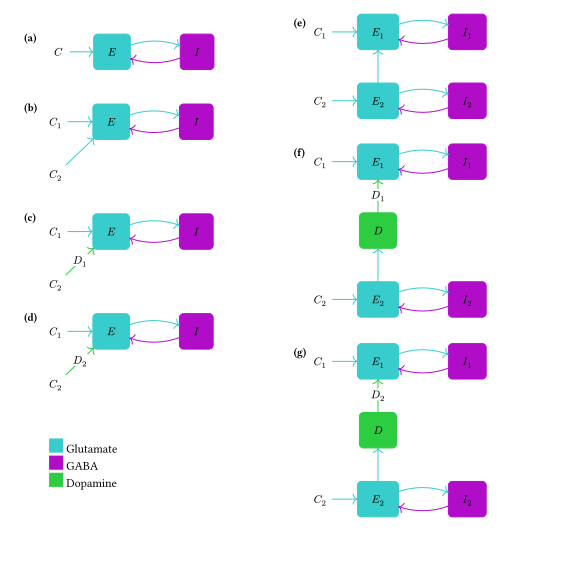
\includegraphics[width=0.75\textwidth]{model_arch.png}
    \caption{Model structure}
\end{figure*}

The auto-associative point attractor was split into two groups: the excitatory group ($E_1$) and the inhibitory group ($I_1$). 
The excitatory group expresses the recalled pattern while the inhibitory group ensures stability. 
The each excitatory group had weights structured to store a set of random binary patterns.
In each simulation the excitatory group received input from two separate cues, either through a glutamate input or a dopamine input. 
The network was setup such that the secondary glutamate or dopamine input was from two coupled groups, one excitatory ($E_2$) and one inhibitory ($I_2$).
The input itself was taken from $E_2$. 
There were three types of potential neurotransmitter action: glutamate, $D_1$, and $D_2$. 

When glutamate was used as a secondary cue, $E_1$ was directly connected to the $E_2$. 
One specific binary pattern stored in $E_2$ was chosen at random to be connected to another specific binary pattern stored in $E_1$. Every on bit in the $E_2$ pattern was mapped in a one-to-one manner to an on bit in $E_1$.

When dopamine was used to influence $E_1$, there was an intermediate dopamine group ($D$) between $E_2$ and $E_1$ so there were no internal dopaminergic synapses in $E_2$, but dopamine could be transmitted to $E_2$.
If $D_1$ was simulated, $E_1$ was modified to have $D_1$ receptors ($s_{D_1} > 0$), and if $D_2$ was simulated, $E_1$ was modified to have $D_2$ receptors ($s_{D_2} > 0$).
However, if $s_{D_2}$ was simulated, the pattern in $E_2$ mapped on bits to off bits in $E_1$ since $D_2$ action was inhibitory.
The model first applied $C_2$ and then $C_1$ to ensure that $C_2$ was a prior cue. 
The simulations tested the preference for a certain cue under different distortion conditions; a healthy control should see that $C_1$ takes priority when distortion is low but $C_2$ takes priority when distortion is high.
Schizophrenic behavior should see a higher tendency to tend towards representing $C_2$ as Bayesian inference is deregulated in a manner that results in prior cues having a larger effect.

As a control, $E_1$ coupled to $E_2$ was simulated with no Bayesian inference to demonstrate how hallucinations could form independently of inference.

quick notes: 
there should be four simulations
control with no bayesian inference where cue is applied immediately to $E_1$
control with no bayesian inference where no cue is applied
(if when no cue is applied, memory never holds, try using a small noisy cue)
one where a cue is applied immediately directly to $E_1$ and then removed
one where no cue is applied to $E_1$ but $E_2$ inputs a cue
pattern switching simulations too

D2 SHOULD BE FIT TO DOPAMINE-GLUTAMATE PAPER
should have svg figure somewhere

maybe analyze manifolds too

\section{Results and Discussion}

\subsection{Control with No Bayesian Inference}
\subsubsection{Cue Applied}
\subsubsection{No Cue Applied}

\subsection{Cues Applied to Same Group}
\subsubsection{Glutamate Based Inference}
\subsubsection{Dopamine Based Inference}

\subsection{Inter-group Cues}
\subsubsection{Glutamate Based Inference}
\subsubsection{Dopamine Based Inference}

\section{Conclusion}

\section{quick notes}
\begin{itemize}
    \item Demonstrate that c2 takes over with high enough distortion
    \item Should have noisy cue/no cue on c1 and c2 input, to trigger hallucinations
\end{itemize}

\bibliographystyle{ieeetr}
\bibliography{refs}

\end{document}
